\begin{figure}[htbp]
  \centering
  \caption{Confronto frente à Melhor Solução Conhecida (MSC: $\lvert\mathcal{A}'\rvert = 9$, $\lvert\mathcal{O}'\rvert = 6\,813$, $f = 757{,}00$) na instância \texttt{B/0013}. A solução inicial do \texttt{AisleBased} parte de $-52$ unidades abaixo da MSC (barra truncada); \texttt{Santos e Baldotto (2025)} estaciona em $-2$ unidades ($6\,811/9 = 756{,}78$); e o \texttt{GVNS} converge em 100\% das sementes (30/30) para $+1$ unidade acima da MSC ($6\,814/9 = 757{,}11$, $\mathrm{RPD} = -0{,}015\%$).}
  \label{fig:novas_msc_comparativo_b0013}
  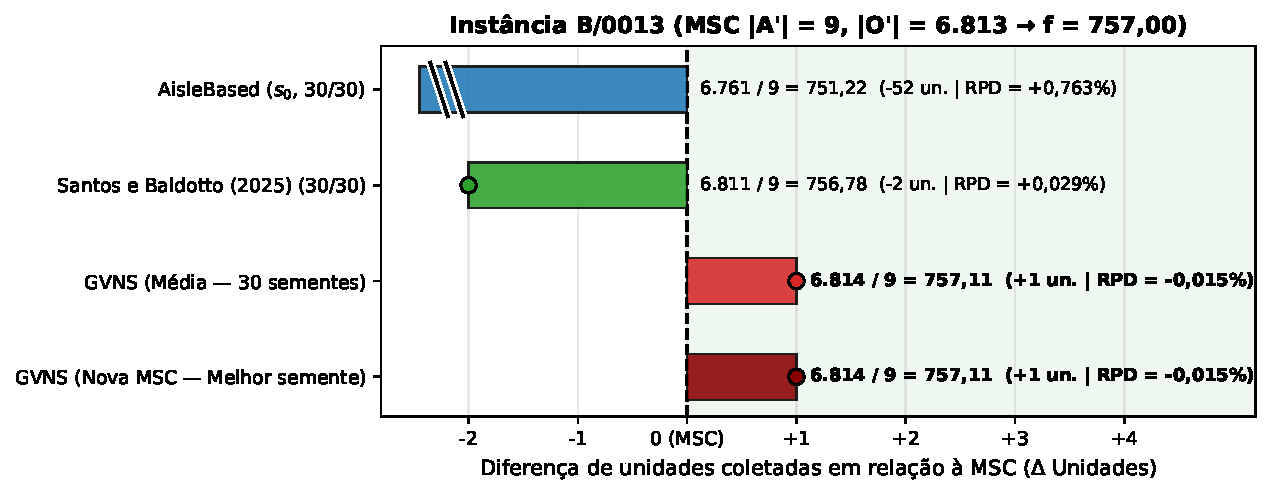
\includegraphics[width=0.85\textwidth]{img/novas_msc_comparativo_b0013.pdf}
  \caption*{\footnotesize Fonte: Elaborado pelo autor, 2026.}
\end{figure}
